% TeX root = ../main.tex
\chapter{Before you copy and paste}

  \section{Why this template?}
  \label{sec:start}
  This template is designed with only one thing in mind. The readability of the script. One of the hardest part in debugging any code, not just $LaTeX$ is squashing bugs. With a good structure to your working directory, you'll be able to read and understand what everything means and where to make changes. Without further due let us start

  \section{How much $LaTeX$ you need?}
  I am under the impression that you might know some $LaTeX$ scripting. Don't worry if you don't, there are plenty of YouTube videos out there. Get just the basics like how to make a simple text document, some math symbols, inline equations, block equations, aligning equations etc. \url{https://latex.js.org/playground.html} is an online playground which will give you a quick introduction.

  \section{Where to start in this template?}
  The directory is setup in a way that almost all the settings are inteh \texttt{config} directory. If you open \texttt{main.tex}, the first thing included is the \texttt{config/packages.tex}. 
  \subsection{\texttt{config/packages.tex}}
  This file imports some of the essential packages that are required. I've added what some of these packages do as comments next to them. Uncomment/add the required packages here. For more details about these packages go to \url{https://www.ctan.org/}\texttt{pkg/\textit{packagename}} and read the documentation there.
  
  \subsection{\texttt{config/options.tex}}
  The next thing imported by \texttt{main.tex} is \texttt{config/options.tex}. This file contains all the settings for the packages imported from \texttt{config/packages.tex}. If you want to specify further options, put all of them into this file. Refer the documentation at \url{https://www.ctan.org} for specific options of the packages.

  \subsection{\texttt{config/colors.tex}}
  This file contains color settings.

  \subsection{\texttt{config/theoremstyle.tex}}
  This file contains the settings to stylize definitions and theorems for your document.

  \subsection{\texttt{config/mathletters.tex}}
  This file contains some shortcuts which helped me typeset math equations.

  \section{Adding content}
  The chapters of the report is supposed to be in the folder \texttt{01Chapters}. Make a tex file for each chapter as it simplifies the content.

  \section{Front Matter}
  Edit the files in \texttt{00Intro} with your details.

  \section{Citations and References}
  Cite whatever you want with \texttt{\/autocite} like \autocite[Theorem~3.14 \pno~69]{papaRudin} and refer things with \texttt{\/autoref}, its way better than \texttt{\/ref}. You can just refer things like \autoref{sec:start} and don't have to do section \ref{sec:start}(Look at the code to see what I mean)

  The bibliography file is set to \texttt{02End/math.bib}, using \texttt{bibsource} in line 8 of \texttt{main.tex}. Edit the \texttt{.bib} file adding your citations. The citationstyle can also be changed. Refer \texttt{biblatex} documentation for this. 

  Remember to run \texttt{biber} if you are working in your local system and not \href{https://www.overleaf.com}{overleaf}.

  \section{Info}
  Fork me on \href{https://github.com/joelsleeba/iisertvm-thesis-template}{GitHub} and contribute to the project.

  \vfill
  \centering
  \reflectbox{\copyright} Joel Sleeba

\newpage
\newpage
\begin{figure}
    \centering
    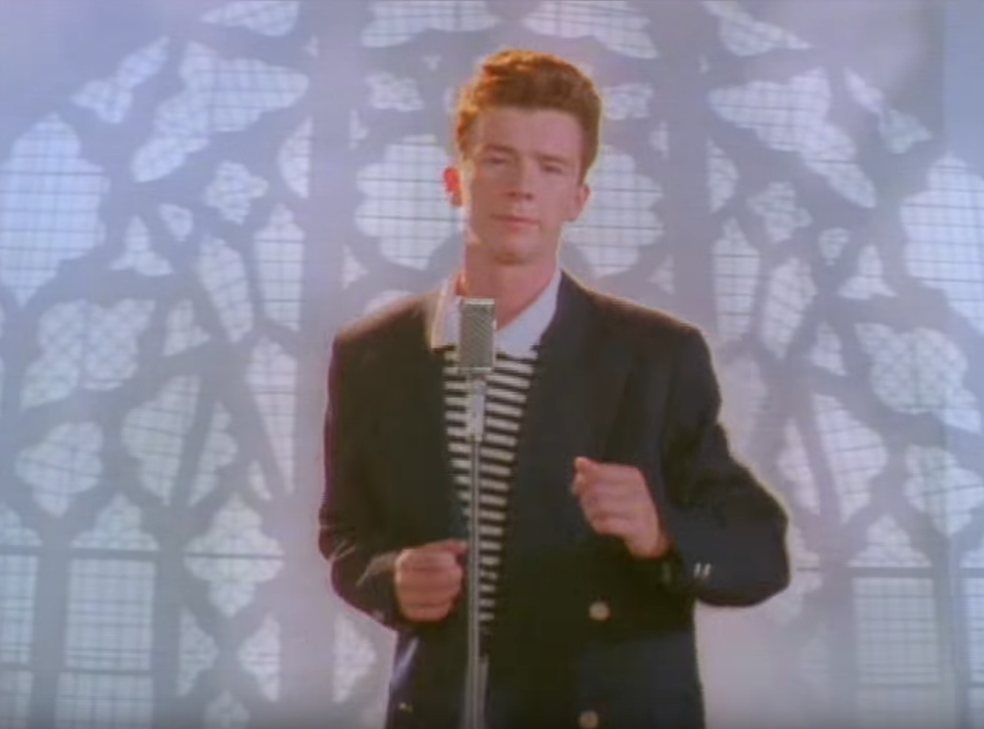
\includegraphics[width=0.6\textwidth]{clickbait}
    \caption{Poor boy needs money. Help him by sending your charitable donations}
    \label{fig:clickbait}
\end{figure}
